% Version 2020
%

\subsection{Introducci\'on}

Los Sistemas de Navegaci\'on Hiperb\'olicos son aquellos que utilizan como t\'ecnica de localizaci\'on de la aeronave la intersecci\'on de hip\'erbolas. Son sistemas de largo alcance, que han sido utilizados en vuelos intercontinentales o transoce\'anicos.

\begin{figure}[!h]
  \centering
\includegraphics[width=0.7\textwidth]{06.radionavegacion/Imagenes/06.01.adf/Hiperbola.gif}
  \caption{Elementos de una hip\'erbola}
  \label{fig:hiperbola}
  \label{!h}
\end{figure}


La hip\'erbola es una de las c\'onicas (elipse, par\'abola, hip\'erbola) y se define como el lugar geom\'etrico de los puntos cuyas diferencias de distancias a dos puntos fijos, denominados focos, es constante. Matem\'aticamente esto se expresa como:

\[\left|{FP}-{F'P}\right|= 2a
\]

Donde los puntos $F$ y $F'$ son los focos de la c\'onica (Figura \ref{fig:hiperbola}), y $2a$ es la distancia entre los dos v\'ertices de las curvas.

El principio de funcionamiento de los sistemas hiperb\'olicos se basa en que la aeronave tenga a borde el equipo necesario para determinar la diferencia de distancias que la separan de dos estaciones fijas situadas en tierra. Para ello se asume que las dos estaciones terrestres, ubicadas en los focos, emiten ondas electromagn\'eticas en todas direcciones. El punto $P$ que representa a la aeronave, recibe las ondas y determina la diferencia de distancias que la separan de las estaciones terrestres.

De esta manera, el operador a bordo de la aeronave, determina en que ``hip\'erbola'' se encuentra, pero no sabe en que punto de la misma est\'a ubicado. 
Para solucionar esto se requiere una hip\'erbola m\'as, lo que se logra
con un sistema de tres estaciones terrestres, 
a fin de minimizar la indeterminaci\'on a dos posibles puntos 
o tres hip\'erbolas para localizar la nave en un \'unico punto. 
Con dos curvas sobra precisi\'on para la localizaci\'on ya que, 
de los dos puntos posibles, uno se desestima por encontrarse muy alejado de la ruta.

Han existido diversos sistemas de navegaci\'on hiperb\'olicos, pero la mayor\'ia no operan actualmente o han sufrido modificaciones. Entre ellos se tiene:
\begin{multicols}{2}
\begin{itemize}
\item GEE

\item LORAN-A
\item  LORAN-B
\item LORAN-C
\item LORAN-D

\item DECCA

\item OMEGA

\item TROPIK

\item MARSHRUT

\item SHORAN (SHOrt Range Air Navigation)
\end{itemize}
\end{multicols}

\begin{figure}[!h]
  \centering
  \subfigure[Principio de ubicaci\'on de la posici\'on por navegaci\'on hiperb\'olica]{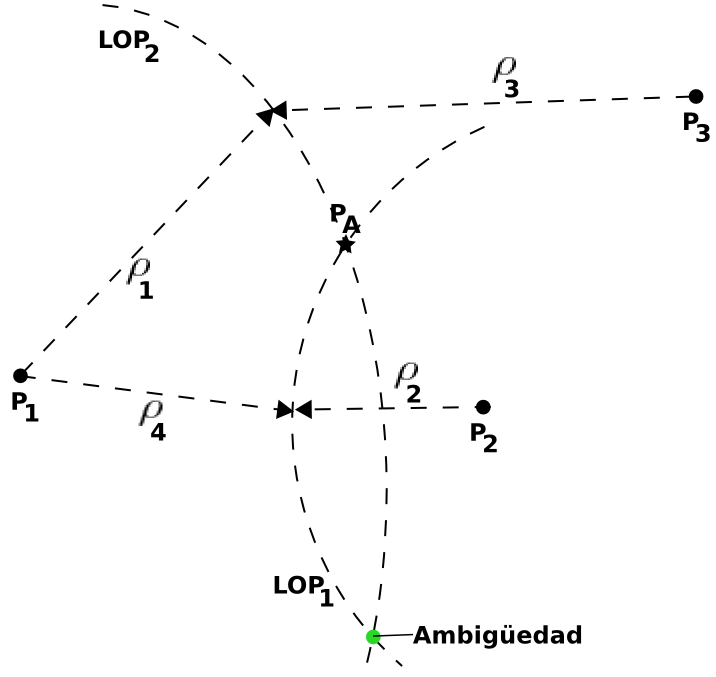
\includegraphics[width=0.4\textwidth]{06.radionavegacion/Imagenes/06.01.adf/hiperbolic-fix.png}   \label{fig:principio.navegacion.hiperbolica}
}
\hspace{1em}
\subfigure[Triángulo de situación]{
  \scalebox{0.80}{
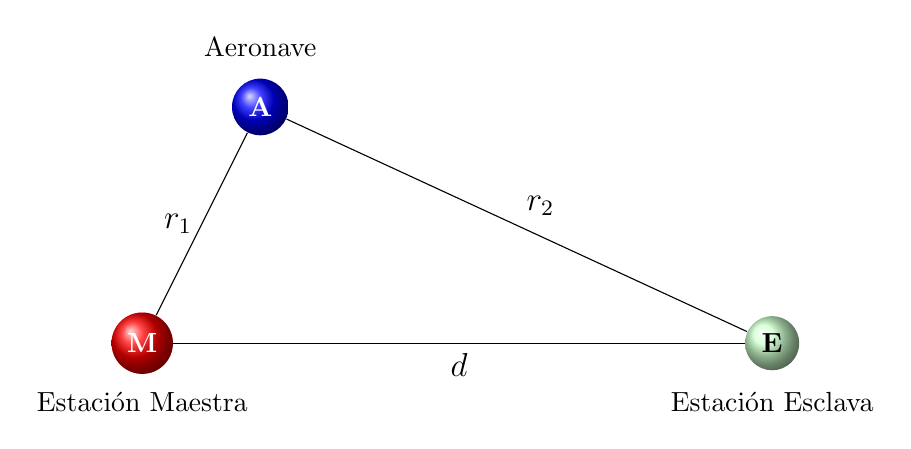
\begin{tikzpicture}[scale=1]
%\usetikzlibrary{snakes}
%\usetikzlibrary{calc}

%  \draw[help lines, green!70, step=0.5] (0,0) grid (9,4);
	% Impulso tiempo t0

	\node[circle, 
				shading=ball, 
				fill=red!50, 
				ball color=red,
				text=white
				] (M) at (0,0) {$\bf M$};

	\node[circle,
				shading=ball, 
				ball color=green!20,
%				text=white
				] (E) at (8,0) {$\bf E$};

	\node[circle,
				shading=ball,
%				ball color=black,
				text=white
				] (A) at (1.5,3) {$\bf A$};

	\draw (M) ++(0.0,-0.5) node[anchor=north] {Estaci\'on Maestra}; 
	\draw (E) ++(0.0,-0.5) node[anchor=north] {Estaci\'on Esclava}; 
	\draw (A) ++(0.0,1.0) node[anchor=north] {Aeronave}; 

	\draw (M) -- (A) node[midway, above,anchor=east] {\large $r_1$};
	\draw (E) -- (A) node[midway, above,anchor=south west] {\large $r_2$};
	\draw (M) -- (E) node[midway, above,anchor=north] {\large $d$};

\end{tikzpicture}
    }
%  \caption{Tri\'angulo de situaci\'on}
  \label{fig:06.triangulo.situacion}
 }
 \caption{Navegaci\'on hiperb\'olica}

\end{figure}


\subsubsection{T\'ecnicas de navegaci\'on hiperb\'olica}

Los sistemas hiperb\'olicos solo pueden determinar diferencias de distancias, para ello se emplean dos t\'ecnicas diferentes:

\begin{description}
\item [T\'ecnica de impulsos-tiempos:] conociendo la velocidad de las ondas electromagn\'eticas, $\mathbf{c}$, se puede relacionar el tiempo medido con la distancia recorrida mediante la expresi\'on:

\[ \Delta\,r = c\,\Delta t
\]

De donde:

\[ r = r_0+c\,\left(t-t_0\right)
\]

%\begin{figure}[!h]
% \end{figure}

Pero la ecuaci\'on encierra una gran dificultad de llevar a la pr\'actica puesto que $t_0$ implica conocer el momento exacto en que se produjo la transmisi\'on del emisor. Este problema desaparece si se considera, en lugar de una distancia determinada a una estaci\'on, una diferencia de distancias a dos estaciones puesto que si ambas transmiten sincronizadas, al efectuarse la diferencia de distancia la inc\'onita $t_0$ desaparece.

Para ver con mas detalle lo anterior, consid\'erese una estaci\'on emisora maestra, $M$  que empieza su emisi\'on en el tiempo $t_0$; otra estaci\'on denominada esclava ubicada a una distancia $d$ de la estaci\'on maestra, recibe esta se\~nal luego de un tiempo $d/c$. Luego de un tiempo $\tau$, denominado ``tiempo de sincronismo'', emite una se\~nal id\'entica a la recibida. 

El receptor en la aeronave ($A$) recibe las se\~nales emitidas por las emisoras maestra y esclava, calculando la diferencia de tiempo entre ambas $\Delta\,t = t_2-t_1$. 

Partiendo de la estaci\'on maestra en el tiempo $t_0$, el impulso tarda un tiempo $t_1-t_0$ en llegar al receptor de la aeronave:

\[t_1-t_0 = \displaystyle \frac{r_1}{c}
\]

Al llegar el impulso de la estaci\'on madre a la esclava, esta luego del tiempo $\tau$, emite el suyo el cual llega en el tiempo $t_2$ al receptor, de esta forma se tiene:

\[
t_2-t_0 = \displaystyle \frac{d}{c}+\tau+\frac{r_2}{c}
\]

Haciendo la diferencia de $t_2-t_1$ seg\'un las expresiones anteriores:

\[
t_2-t_1 = t_0 + \displaystyle \frac{d}{c}+\tau+\frac{r_2}{c} - t_0 -\frac{r_1}{c} = \tau+\frac{d+r_2-r_1}{c} = \tau+\frac{d+\Delta\,r}{c}
\]

Finalmente:

\[
\Delta\,t = \tau+\frac{d+\Delta\,r}{c}
\]

Esta expresi\'on implica que a cada incremento de tiempo ($\Delta t$) le corresponde uno de distancia ($\Delta r$), con los par\'ametros $d$, $c$ y $\tau$ conocidos.

Pero debe recordarse algo, en lugar de considerar hip\'erbolas que son curvas planas, este m\'etodo ubica al receptor en un hiperboloide de revoluci\'on. Por esto deben hacerse correcciones por la curvatura y forma de la tierra.


\item [T\'ecnica de onda continua-fases:]

En esta t\'ecnica la emisi\'on es de forma continua a diferencia de la anterior que es por pulsos y que el par\'ametro que se mide es la diferencia de fases.

Se utilizan dos emisores omnidireccionales con un sincronismo de fases entre sus se\~nales. El receptor recibe a ambas se\~nales con una diferencia de fase, que depende de la distancia de la aeronave a cada una de las emisoras. De esta manera se determina la hip\'erbola donde se encuentra el receptor.

Conociendo la longitud de onda $\lambda$ se puede obtener la distancia recorrida seg\'un la fase medida: 

\[\Delta r = \lambda \,\Delta \phi \quad \Longrightarrow r = r_0 +\lambda \,\left( \phi - \phi_0 \right) \]

Aqui se presenta una dificultad porque el receptor necesita conocer $ \phi_0$, la fase exacta en que se produjo la transmisi\'on.

El proceso se realiza de la siguiente forma, la estaci\'on maestra ubicada en $M$ emite su se\~nal continua con frecuencia $f_1$ (longitud de onda $\lambda_1$) y origen de fases $ {\phi_1}_0$. La estaci\'on esclava en $E$ recibe esta se\~nal y transmite la suya con frecuencia $f_2$ y fase inicial $ {\phi_2}_0$. La frecuencia $f_2$ es diferente de la $f_1$ para que el receptor pueda separar facilmente las se\~nales.

La antena de la aeronave recibe ambas se\~nales $f_1$ y $f_2$ con fases $\phi_1$ y $\phi_2$ diferentes a las de salida, cuyos valores son:

\[
\phi_1 = {\phi_1}_0 + \displaystyle \frac{r_1}{\lambda_1} \qquad
\phi_2 = {\phi_2}_0 + \displaystyle \frac{r_2}{\lambda_2} 
\]

Para poder comparar estas se\~nales se usa el artificio de una frecuencia com\'un, $f_c$, con longitud de onda $\lambda_c$ que resulta de multiplicar a cada una de las frecuencias anteriores por un n\'umero entero $n_1$ y $n_2$, respectivamente:

\[
f_c = n_1\,f_1 = n_2\,f_2
\]

Cuando se multiplica una frecuencia por un n\'umero, se hace lo mismo con su fase, por lo que las expresiones anteriores vistas desde esta frecuencia com\'un, quedan:

\[
\theta_1 = n_1\,\phi_1 = n_1\,{\phi_1}_0 + \displaystyle \frac{n_1\,r_1}{\lambda_1} \qquad
\theta_2 = n_2\,\phi_2 = n_2\,{\phi_2}_0 + \displaystyle \frac{n_2\,r_2}{\lambda_2} 
\]

Restando la diferencia de las fases:

\[
\Delta\,\theta = \theta_1-\theta_2 = n_1\,{\phi_1}_0 + \displaystyle \frac{n_1\,r_1}{\lambda_1} -  n_2\,{\phi_2}_0 - \displaystyle \frac{n_2\,r_2}{\lambda_2} 
\]

El sincronismo de fase entre la estaci\'on maestra y la esclava debe realizarse de forma que se cumpla lo siguiente:

\begin{itemize}
\item La diferencia de fases iniciales multiplicadas por su entero respectivo debe mantenerse constante: $n_1\,{\phi_1}_0- n_2\,{\phi_2}_0= cte$

\item El ajuste de sincronismo que realiza la estaci\'on esclava cumple, en la prolongaci\'on de la l\'inea que la une con la maestra pero en el lado de la maestra, que la diferencia de fases en la aeronave sea nula: 

Para $r_1=0$ y $r_2=d$ se cumple que $\Delta\,\theta = \theta_1-\theta_2 =0$

\end{itemize}

Sabiendo que para un lado se cumple $c = f_c\,\lambda_c = f_1\,\lambda_1$ y como $f_c=n_1\,f_1$, entonces $n_1f_1\lambda_c = f_1\lambda_1$, por lo que $n_1\lambda_c=\lambda_1$ o $\displaystyle \frac{n_1}{\lambda_1}=\frac{1}{\lambda_c}$.

De la misma manera se obtiene $\displaystyle \frac{n_2}{\lambda_2}=\frac{1}{\lambda_c}$.

Volviendo a la diferencia de fases de la frecuencia com\'un:

\[
\Delta\,\theta = n_1\,{\phi_1}_0- n_2\,{\phi_2}_0 +  \displaystyle \frac{n_1\,r_1}{\lambda_1}  - \displaystyle \frac{n_2\,r_2}{\lambda_2}= cte + \frac{\Delta r}{\lambda_c}
\]

Trabajando con la expresi\'on anterior se llega a que:

\[
\Delta \theta = \displaystyle \frac{d+\Delta r}{\lambda_c}
\]

Surge un problema adicional, esta expresi\'on solo resuelve el incremento de fase dentro de una longitud de onda determinada pero se desconoce dentro de cual. 
Esto resulta en una indeterminaci\'on m\'ultiple, ya que el \'angulo real ser\'a un n\'umero entero de longitudes de onda m\'as el desfase obtenido de la ecuaci\'on anterior. 
La indeterminaci\'on ser\'a mayor cuanto mayor sea la frecuencia de la se\~nal radiada (menor $\lambda$). 
El inconveniente se soluciona con otra t\'ecnica conocida como del n\'umero de longitudes de onda completas.


\end{description}


\subsection{LORAN}
\label{sec:06.loran}

%Ver la siguiente pagina, de donde sacaron la informacion los de Alaca
%http://jproc.ca/hyperbolic/loran_c.html


El \textbf{LORAN} (del ingl\'es LOng RAnge Navigation, navegaci\'on de largo alcance) es un sistema de ayuda a la navegaci\'on electr\'onica de tipo hiperb\'olico
 de largo alcance, que opera en baja y media frecuencia. 

Utiliza el intervalo transcurrido entre la recepci\'on de se\~nales de radio transmitidas desde tres o m\'as transmisores para determinar la posici\'on del receptor. 

Desarrollado a principios de la II Guerra Mundial, el LORAN fue el primer sistema de navegaci\'on basado en la llegada diferenciada de se\~nales de radio. Fue concebido por el laboratorio de Radiaci\'on de MIT. LORAN fue, tambi\'en, el primer sistema de posicionamiento capaz de funcionar bajo cualquier condici\'on climatol\'ogica pero es solamente bidimensional (latitud y longitud).

\begin{figure}[!tbh]
  \centering
  \subfigure[Interior de la instalaci\'on emisora]{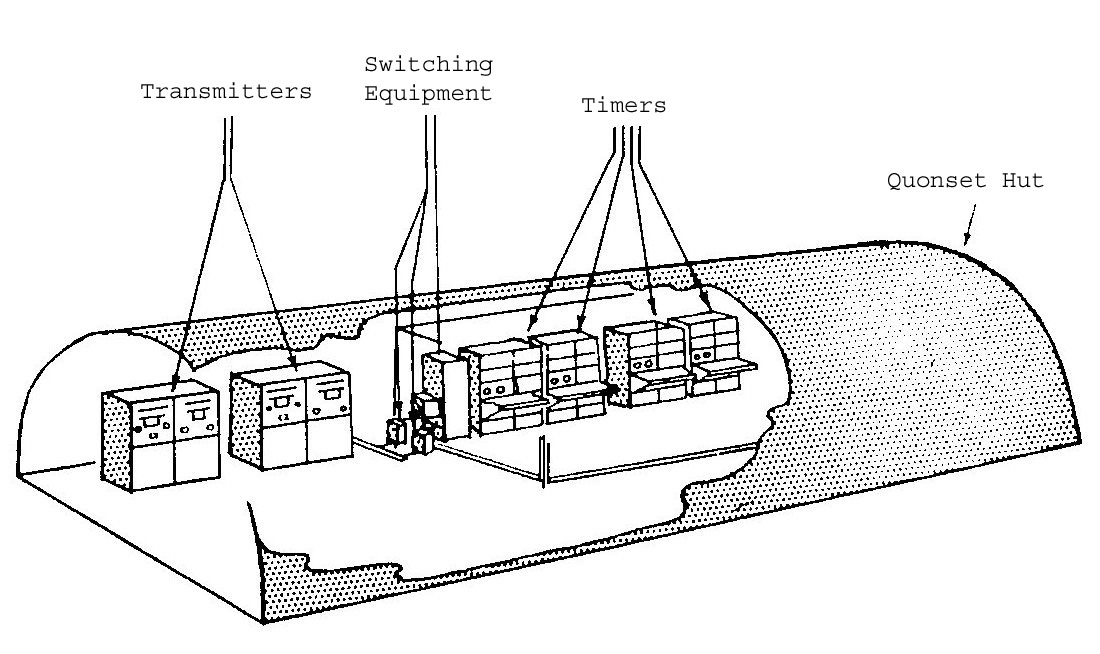
\includegraphics[height=5.5cm]{06.radionavegacion/Imagenes/06.01.adf/LORAN-Equip-Hut_.jpg}}
  \subfigure[Vista de estaci\'on emisora]{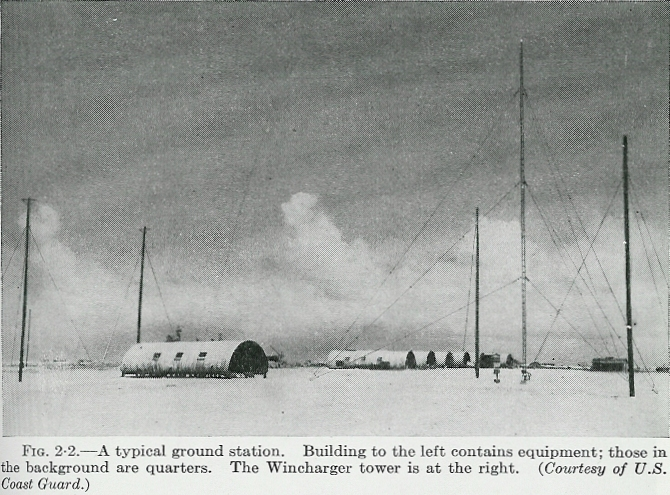
\includegraphics[height=5.5cm]{06.radionavegacion/Imagenes/06.01.adf/LORAN-A_1940-instalacion-terrestre.jpg}}
  \caption{Instalaciones de LORAN-A \protect\cite{Historia_LORAN} }
\end{figure}

 El sistema emisor LORAN se compone de una estaci\'on maestra y otras esclavas. La maestra emite de forma regular una peque\~na se\~nal, que es repetida por la esclava, controlada por radio desde la maestra.
En la Figura \ref{fig:06.loran.cadenas} puede observarse la configuraci\'on t\'ipica de cadenas LORAN (Maestra + Esclavas) y una cadena ubicada en USA.

 Ambas se\~nales se reciben en el barco o avi\'on, se amplifican y se registran. Los circuitos del receptor est\'an dispuestos de forma que la distancia entre las se\~nales corresponda a la diferencia de tiempos de llegada de las se\~nales de ambas estaciones. El receptor posee adem\'as un dispositivo temporizador electr\'onico que permite medir dicha diferencia en microsegundos (millon\'esimas de segundo). 

En la Figura \ref{fig:06.loran.vista.detallada.pulso.y.gri} puede observase un detalle del pulso emitido en la se\~nal LORAN y del \ac{GRI}.

% \begin{landscape}
   \begin{figure}[!h]
     \centering
     \subfigure[Configuraciones t\'ipicas de cadenas LORAN]{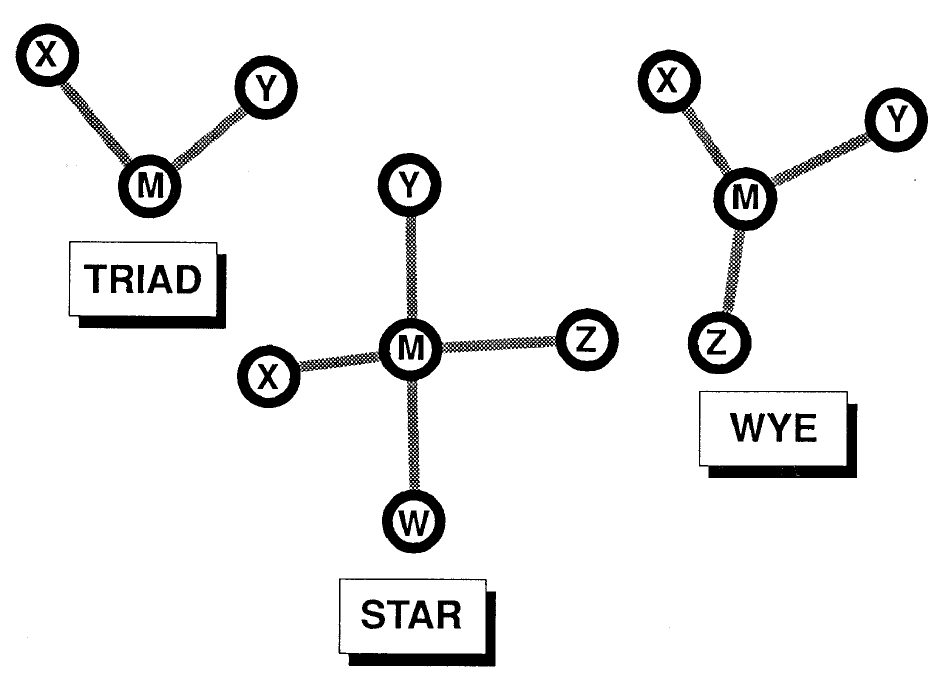
\includegraphics[width=0.5\textwidth]{06.radionavegacion/Imagenes/06.01.Loran/configuracion_cadenas_Loran.png}}
     \subfigure[Cadena LORAN GRI 9960]{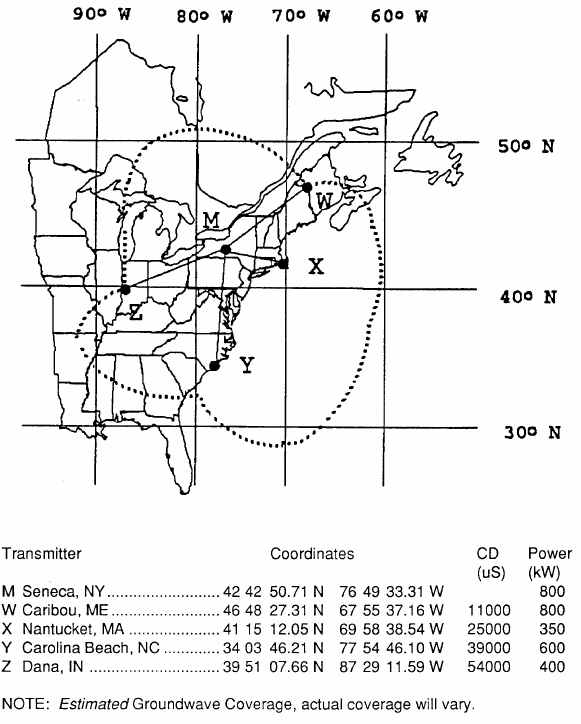
\includegraphics[width=0.5\textwidth]{06.radionavegacion/Imagenes/06.01.Loran/Loran_cadena_GRI_9960.png}}
     \caption{Cadenas LORAN \protect\cite{LoranC_user_book}}
     \label{fig:06.loran.cadenas}
   \end{figure}

% \end{landscape}
 
% \begin{figure}[!h]
%      \centering
%      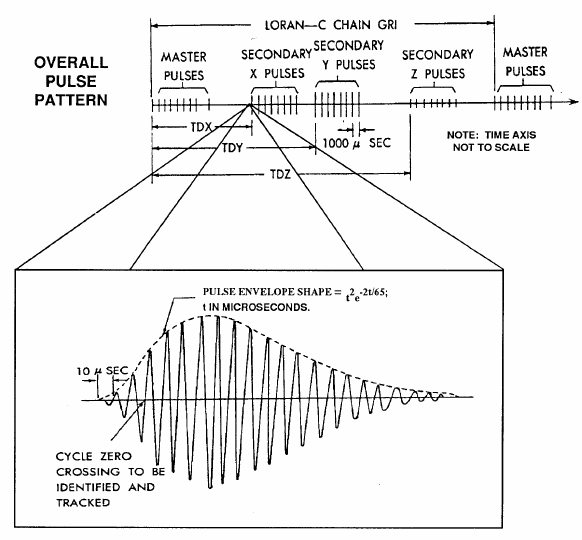
\includegraphics[width=\textwidth]{06.radionavegacion/Imagenes/06.01.Loran/Loran_vista_detallada_pulso_+GRI.png}
%      \caption{Vista detallada de un pulso y de GRI \protect\cite{LoranC_user_book}}
%      \label{fig:06.loran.vista.detallada.pulso.y.gri}
%    \end{figure}





Como las ondas de radio viajan a una velocidad aproximadamente constante de 3$ \times 10^8$ m/segundo, la ubicaci\'on de todos los puntos en los que las se\~nales de las dos estaciones est\'an separadas un determinado intervalo de tiempo se puede representar mediante una curva concreta que es una hip\'erbola (Figura \ref{fig:LORAN_hiperbolas}). El navegante dispone de un mapa con muchas de estas curvas, denominadas curvas de posici\'on LORAN, y tras determinar la diferencia de tiempos, por ejemplo, 3 $\mu$segundos, sabe que la posici\'on de su nave se halla en alg\'un punto de la curva de 3 $\mu$segundos del mapa. Sintonizando una pareja de emisores LORAN y repitiendo este proceso, el navegante es capaz de detectar otra curva que represente la posici\'on de la nave, la posici\'on real de la aeronave se halla en la intersecci\'on de las dos curvas LORAN. 


\begin{figure}[!h]
  \centering
  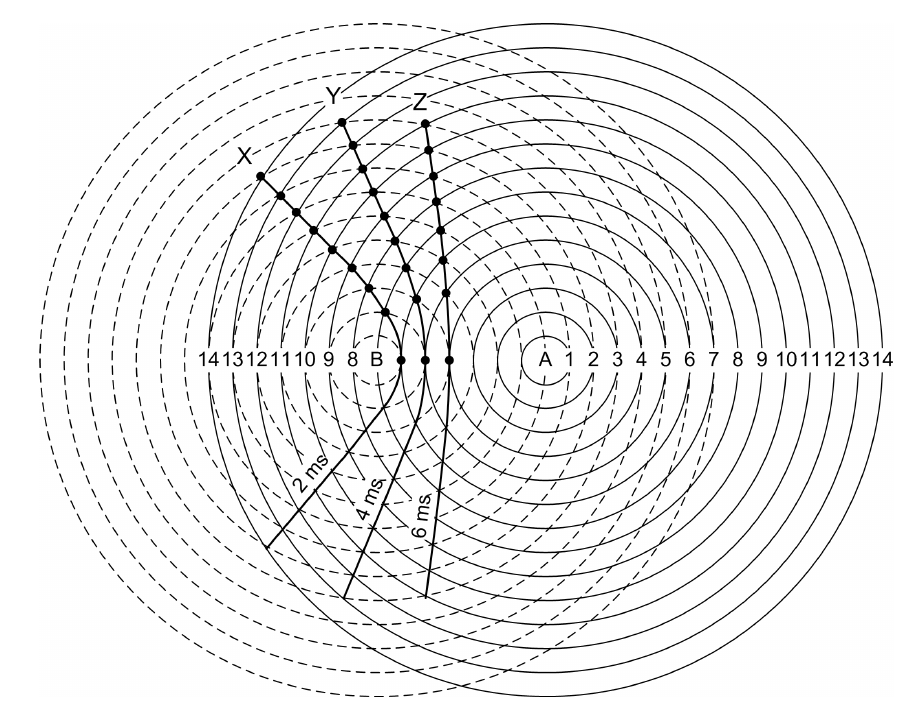
\includegraphics[width=0.8\textwidth ]{06.radionavegacion/Imagenes/06.01.Loran/06_Loran_intersecciones.png}
  \caption{Mapa de hip\'erbolas del sistema LORAN, (A) Estación Maestra, (B) Estación Esclava, $\tau=1$mseg, tiempos en mseg \protect\cite{tooley2017aircraft}}
  \label{fig:LORAN_hiperbolas}
\end{figure}


Este sistema pose\'ia un alcance \'util de unos 2592,8 km (1400 nm) por la noche y unos 1296,4 km (700 nm) de d\'ia,
ver Figuras \ref{fig:06.LoranC.alcances}. 
%Las se\~nales se emitían generalmente en la banda de frecuencias de 1,8 a 2,0 MHz. 
Sirvi\'o tanto para marcar y mantener un rumbo, como para fijar la posici\'on, y presentaba la ventaja de ser independiente de las condiciones meteorol\'ogicas. Su exactitud oscilaba entre unos centenares de metros y unos pocos kil\'ometros, dependiendo del equipo utilizado y de la distancia entre la nave y la emisora. 

La versi\'on m\'as moderna fu\'e LORAN-C que oper\'o en frecuencias del espectro electromagn\'etico entre 90 y 110 Khz (la portadora es 100 kHz para todas las estaciones). El sistema LORAN fu\'e utilizado en muchos pa\'ises, entre ellos los Estados Unidos de Am\'erica, Jap\'on y varios pa\'ises europeos. Rusia utiliz\'o un sistema casi id\'entico llamado CHAYKA, que emple\'o la misma banda de frecuencias. 

\begin{figure}[!h]
  \centering
  \subfigure[Alcance de VOR y DME]{ 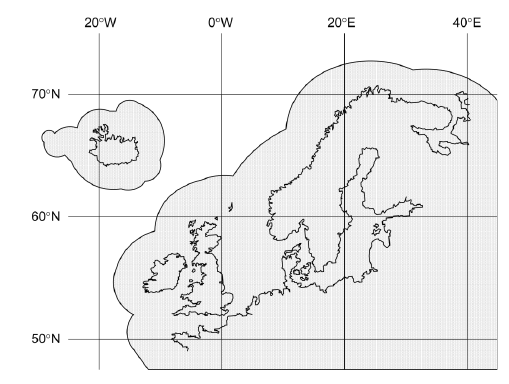
\includegraphics[height=18em]{06.radionavegacion/Imagenes/06.01.Loran/06_VOR+DME_cobertura_marDelNorte.png}}\hspace{1em}
  \subfigure[Alcance de Loran C]{ 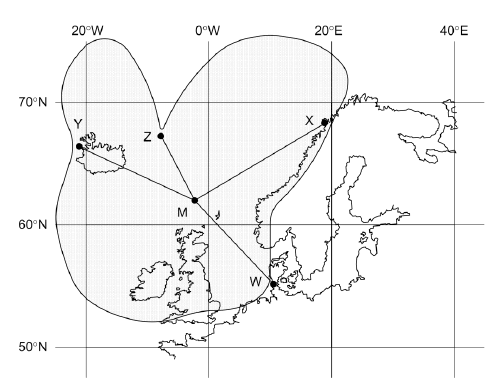
\includegraphics[height=18em]{06.radionavegacion/Imagenes/06.01.Loran/06_LoranC_cobertura_marDelNorte.png}}
  \caption{Comparación de alcances de sistema VOR+DME y Loran-C \protect\cite{tooley2017aircraft}}
  \label{fig:06.LoranC.alcances}
\end{figure}



% From  Tooley Aircraft communications
%
% The intention for a Loran-C system is to only use ground waves for navigation purposes; sky waves are filtered out with pulse timing techniques. The approximate time taken for a transmitted wave to reflect off the ionosphere is 30 ms; since the pulse duration is 270 ms some of the transmitted pulse can be expected to be reflected from the ionosphere. To avoid this, a specific peak within the pulse is selected as the indexing pulse. This is the third peak within the pulse and represents approximately 50% of the maximum amplitude.

% Signals are transmitted from the master station as a group of nine pulses; secondary stations transmit eight pulses, see Figure 14.6. Groups of pulses from each of the chains are transmitted within the range of 10–25 groups per second. Each pulse is spaced at 1 ms intervals; the ninth pulse from the master station occurs after a 2 ms delay. The specific timing interval of the group of pulses (starting and finishing with the master pulses) is referred to as the group repetition interval, or GRI. This time interval is used as the basis of identifying the chain, e.g. a chain with
% GRI of 99,600 microseconds is identified as ``9960''.

% The first group of nine pulses from the master station is received at different times by each of the secondary stations due to the varying baseline distances between respective stations. The secondary stations transmit their pulse groups after predetermined time delays, referred to as the coding delay. The total time for the pulse to travel over the baseline together with the secondary station’s coding delay is called the emission delay. 

% Operational aspects associated with Loran-C include:
% electromagnetic interference affecting the signal, e.g. from power lines loss of one station affecting the area of
% coverage local weather conditions (particularly electrical storms) affecting the signal. 

% In addition to master and secondary stations, monitoring stations are deployed to sample the chain’s signal strength, timing and pulse shape.

% In the event that any of these are outside a specified limit, an alert signal, known as a blink, is coded into the pulse groupings.

\begin{minipage}[c]{0.65\linewidth}
  El Loran-C utiliza ondas terrestres únicamente para fines de
  navegación pero las ondas del cielo pueden interferir por lo cual se
  las filtra con técnicas de sincronización de pulsos.  Una onda
  transmitida tarda en reflejarse en reflejarse en la ionosfera
  aproximadamente 30 mseg, el pulso de Loran-C es de 270 mseg por lo
  que se puede esperar que parte del pulso transmitido se refleje
  desde la ionosfera.  Para evitar esto se selecciona un pico
  específico dentro del pulso como ``\emph{pulso de indexación}'' el
  cual es el tercer pico dentro del pulso y representa aproximadamente
  el 50\% de la amplitud máxima, ver Figura \ref{fig:06.LoranC.formato.pulsos}.
\end{minipage}\hspace{1em}
\begin{minipage}[c]{0.30\linewidth}
  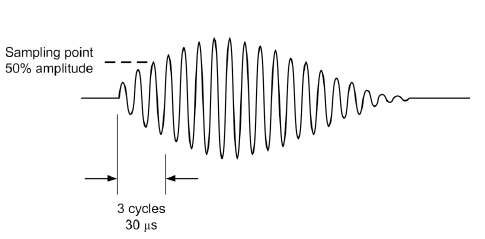
\includegraphics[width=\linewidth]{06.radionavegacion/Imagenes/06.01.Loran/06_LoranC_pulso_formato.png}
  \captionof{figure}{Formato de pulso de Loran-C \protect\cite{tooley2017aircraft}}
  \label{fig:06.LoranC.formato.pulsos}

\end{minipage}

Desde la estación Maestra las señales se transmiten  como un grupo de nueve pulsos mientras que las estaciones secundarias transmiten ocho pulsos, Figura \ref{fig:06.LoranC.secuencia.pulsos}. Los grupos de pulsos de cada una de las cadenas se transmiten dentro del rango de 10 a 25 grupos por segundo. Cada pulso está espaciado a intervalos de 1 mseg; el noveno pulso de la estación maestra ocurre después de un retraso de 2 mseg. El intervalo de tiempo específico del grupo de pulsos (comenzando y terminando con los pulsos maestros) se denomina Intervalo de Repetición de Grupo o Group Repetition Interval (GRI). Este intervalo de tiempo se utiliza como base para identificar la cadena. 
%p. Ej. una cadena con el GRI de 99,600 microsegundos se identifica como `` 9960 ''.

\begin{figure}[!h]
  \centering
  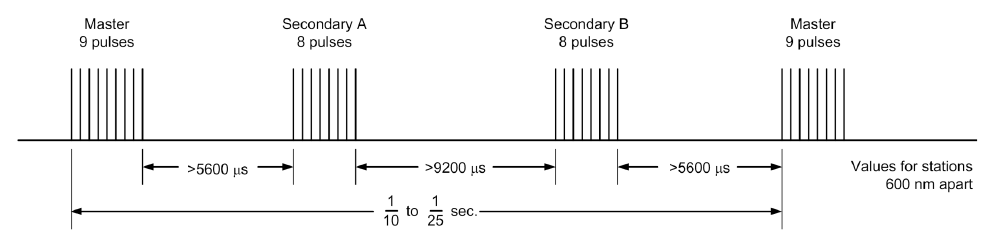
\includegraphics[width=\linewidth]{06.radionavegacion/Imagenes/06.01.Loran/06_LoranC_pulsos_secuencia.png}
  \caption{Intervalo de Repetición de Grupo (GRI) de Loran-C \protect\cite{tooley2017aircraft}}
  \label{fig:06.LoranC.secuencia.pulsos}
\end{figure}

El primer grupo de nueve pulsos de la estación maestra es recibido en diferentes momentos por cada una de las estaciones secundarias debido a las diferentes distancias de línea de base entre las respectivas estaciones. Las estaciones secundarias transmiten sus grupos de pulsos después de retardos de tiempo predeterminados, denominados retardo de codificación. El tiempo total que tarda el pulso en viajar sobre la línea de base junto con el retardo de codificación de la estación secundaria se denomina retardo de emisión.

Los aspectos operativos asociados con Loran-C incluyen:
\begin{itemize}
\item Interferencia electromagnética que afecta a la señal, p. ej. por la presencia de líneas eléctricas.
\item Pérdida de la señal de  una estación que afecta el área
  de cobertura
\item Condiciones meteorológicas severas (particularmente tormentas eléctricas) que afecten a la señal.

\end{itemize}

Además de las estaciones maestra y secundaria se emplean  estaciones de monitoreo  para muestrear la intensidad de la señal de la cadena, el tiempo y la forma del pulso emitido.
Si alguno de estos parámetros se encuentre fuera de un límite especificado, se codifica una señal de alerta, conocida como {\bf blink} (parpadeo) en las agrupaciones de pulsos.



A fin de proporcionar una protección contra la interferencia de fuentes externas y también reducir la contaminación de la onda de tierra 
%de los pulsos transmitidos después 
de las ondas celestes,
% de los pulsos precedentes 
se empleó la codificaci\'on por fase de los pulsos. 
Dado que la onda de cielo del primer pulso llega al receptor al mismo tiempo que la onda de tierra del segundo pulso por lo que esta contaminación 
por ondas del cielo  sin codificación de fase anularía el efecto de muestrear solo la onda terrestre, degradando así la precisión inherente del sistema.

Además, el uso de la codificación de fase también proporciona al receptor la información lógica necesaria para la búsqueda automática de las señales maestra y esclavas. La búsqueda automática se puede utilizar por conveniencia o cuando la relación señal / ruido de las señales recibidas impide la identificación visual.

 
% El uso de pulsos codificados por fase por parte del sistema proporciona una medida de protección contra la interferencia de fuentes externas y también reduce la contaminación de la onda terrestre de los pulsos transmitidos después de las ondas celestes de los pulsos precedentes; es decir, la onda del cielo del primer pulso llega al mismo tiempo que la onda de tierra del segundo pulso. La contaminación por ondas del cielo precedentes sin codificación de fase anularía el efecto de muestrear solo la onda terrestre, degradando así la precisión inherente del sistema. El uso de la codificación de fase también proporciona al receptor la información lógica necesaria para la búsqueda automática de las señales maestra y esclava. La búsqueda automática se puede utilizar por conveniencia o cuando la relación señal / ruido de las señales recibidas impide la identificación visual.


%Within each of these multi-pulse groups from the master and slave stations, the phase of the RF carrier is changed with respect to the pulse envelope in a systematic manner from pulse-to-pulse. The phase of each pulse in an eight or nine-pulse group is changed in accordance with a prescribed code so that it is either in phase (+) or 180? out of phase (-) with a stable 100 kc/s reference signal. The phase code used at a master station is different from the phase code used at a slave, but all slave stations use the same code and currently (1962) all LORAN-C chains use the same code. The sequence utilized in a typical LORAN-C star chain is given below:

Para realizar la codificaci\'on anterior,  la fase de la portadora de RF se cambia con respecto a la envolvente de pulso de manera sistemática de pulso a pulso. 
La secuencia utilizada en una típica cadena LORAN-C se muestra en la Tabla \ref{tab:06.Loran.C.secuencia.cambio.fase}.
La fase de cada pulso en un grupo de ocho o nueve pulsos se cambia de acuerdo con un código prescrito para que esté en fase indicado con el s\'imbolo (+) o 180º fuera de fase indicado con el s\'imbolo (-), con una señal de referencia estable de 100 kHz. 
El código de fase en una estación maestra es diferente del de una esclava, ver 
Tabla \ref{tab:06.Loran.C.secuencia.cambio.fase}.


\begin{table}[!h]
  \centering
\caption{Secuencia de cambio de fase Loran-C \protect\cite{Loran1962}}
\label{tab:06.Loran.C.secuencia.cambio.fase}
% ver pagina 69 de la referencia
  \begin{tabular}{lcccc} \hline
  &MASTER &X-SLAVE& Y-SLAVE& Z-SLAVE \\ \hline
Primer per\'iodo repetici\'on &+ - - +++++ &+ - + - ++- - &+ - + - ++ - - &+ - + - ++ - - \\ 
Segundo per\'iodo repetici\'on &++ - - +-+- &+++++ - - + &+++++ - -+ &+++++ - - + \\
Tercer per\'iodo repetici\'on & \multicolumn{4}{c}{Idem Primer per\'iodo repetici\'on}\\
Cuarto per\'iodo repetici\'on & \multicolumn{4}{c}{Idem Segundo per\'iodo repetici\'on}\\
& \multicolumn{4}{c}{Etc.} \\ \hline
\end{tabular}
\end{table}

%The use of phase-coded pulses by the system provides a measure of protection against interference from outside sources and also reduces contamination of the groundwave of pulses transmitted subsequent to skywaves from preceding pulses; i.e., skywave of the first pulse arriving at the same time as the groundwave of the second pulse. Contamination by preceding skywaves without phase coding would nullify the effect of sampling only the groundwave, thereby degrading the inherent accuracy of the system. The use of phase coding also provides the receiver with necessary logical information for automatic search for the master and slave signals. Automatic search can be utilized for convenience or when the signal- to-noise ratio of the received signals precludes visual identification.




\begin{landscape}


\Informacion{¿El fin del LORAN?}{

  \begin{small}
    El uso de LORAN ha dejado de ser utilizado al ser reeplazado por
    GPS. Sin embargo, debido a la interferencia que se puede producir
    en \'este \'ultimo sistema se ha estudiado la posibilidad de
    mejorar y volver a popularizar este sistema mediane el eLORAN. Ver
    el siguiente art\'iculo 
      \href{https://rntfnd.org/2018/06/06/russia-china-upgrading-loran-eloran-systems/}{\bf
        Russia, China Upgrading Loran/ eLoran Systems?}
%	\href{https://rntfnd.org/2020/08/27/eloran-and-aviation-aviation-policy-news/}{}
  \end{small}
}






  \begin{figure}[!tbh]
    \centering
    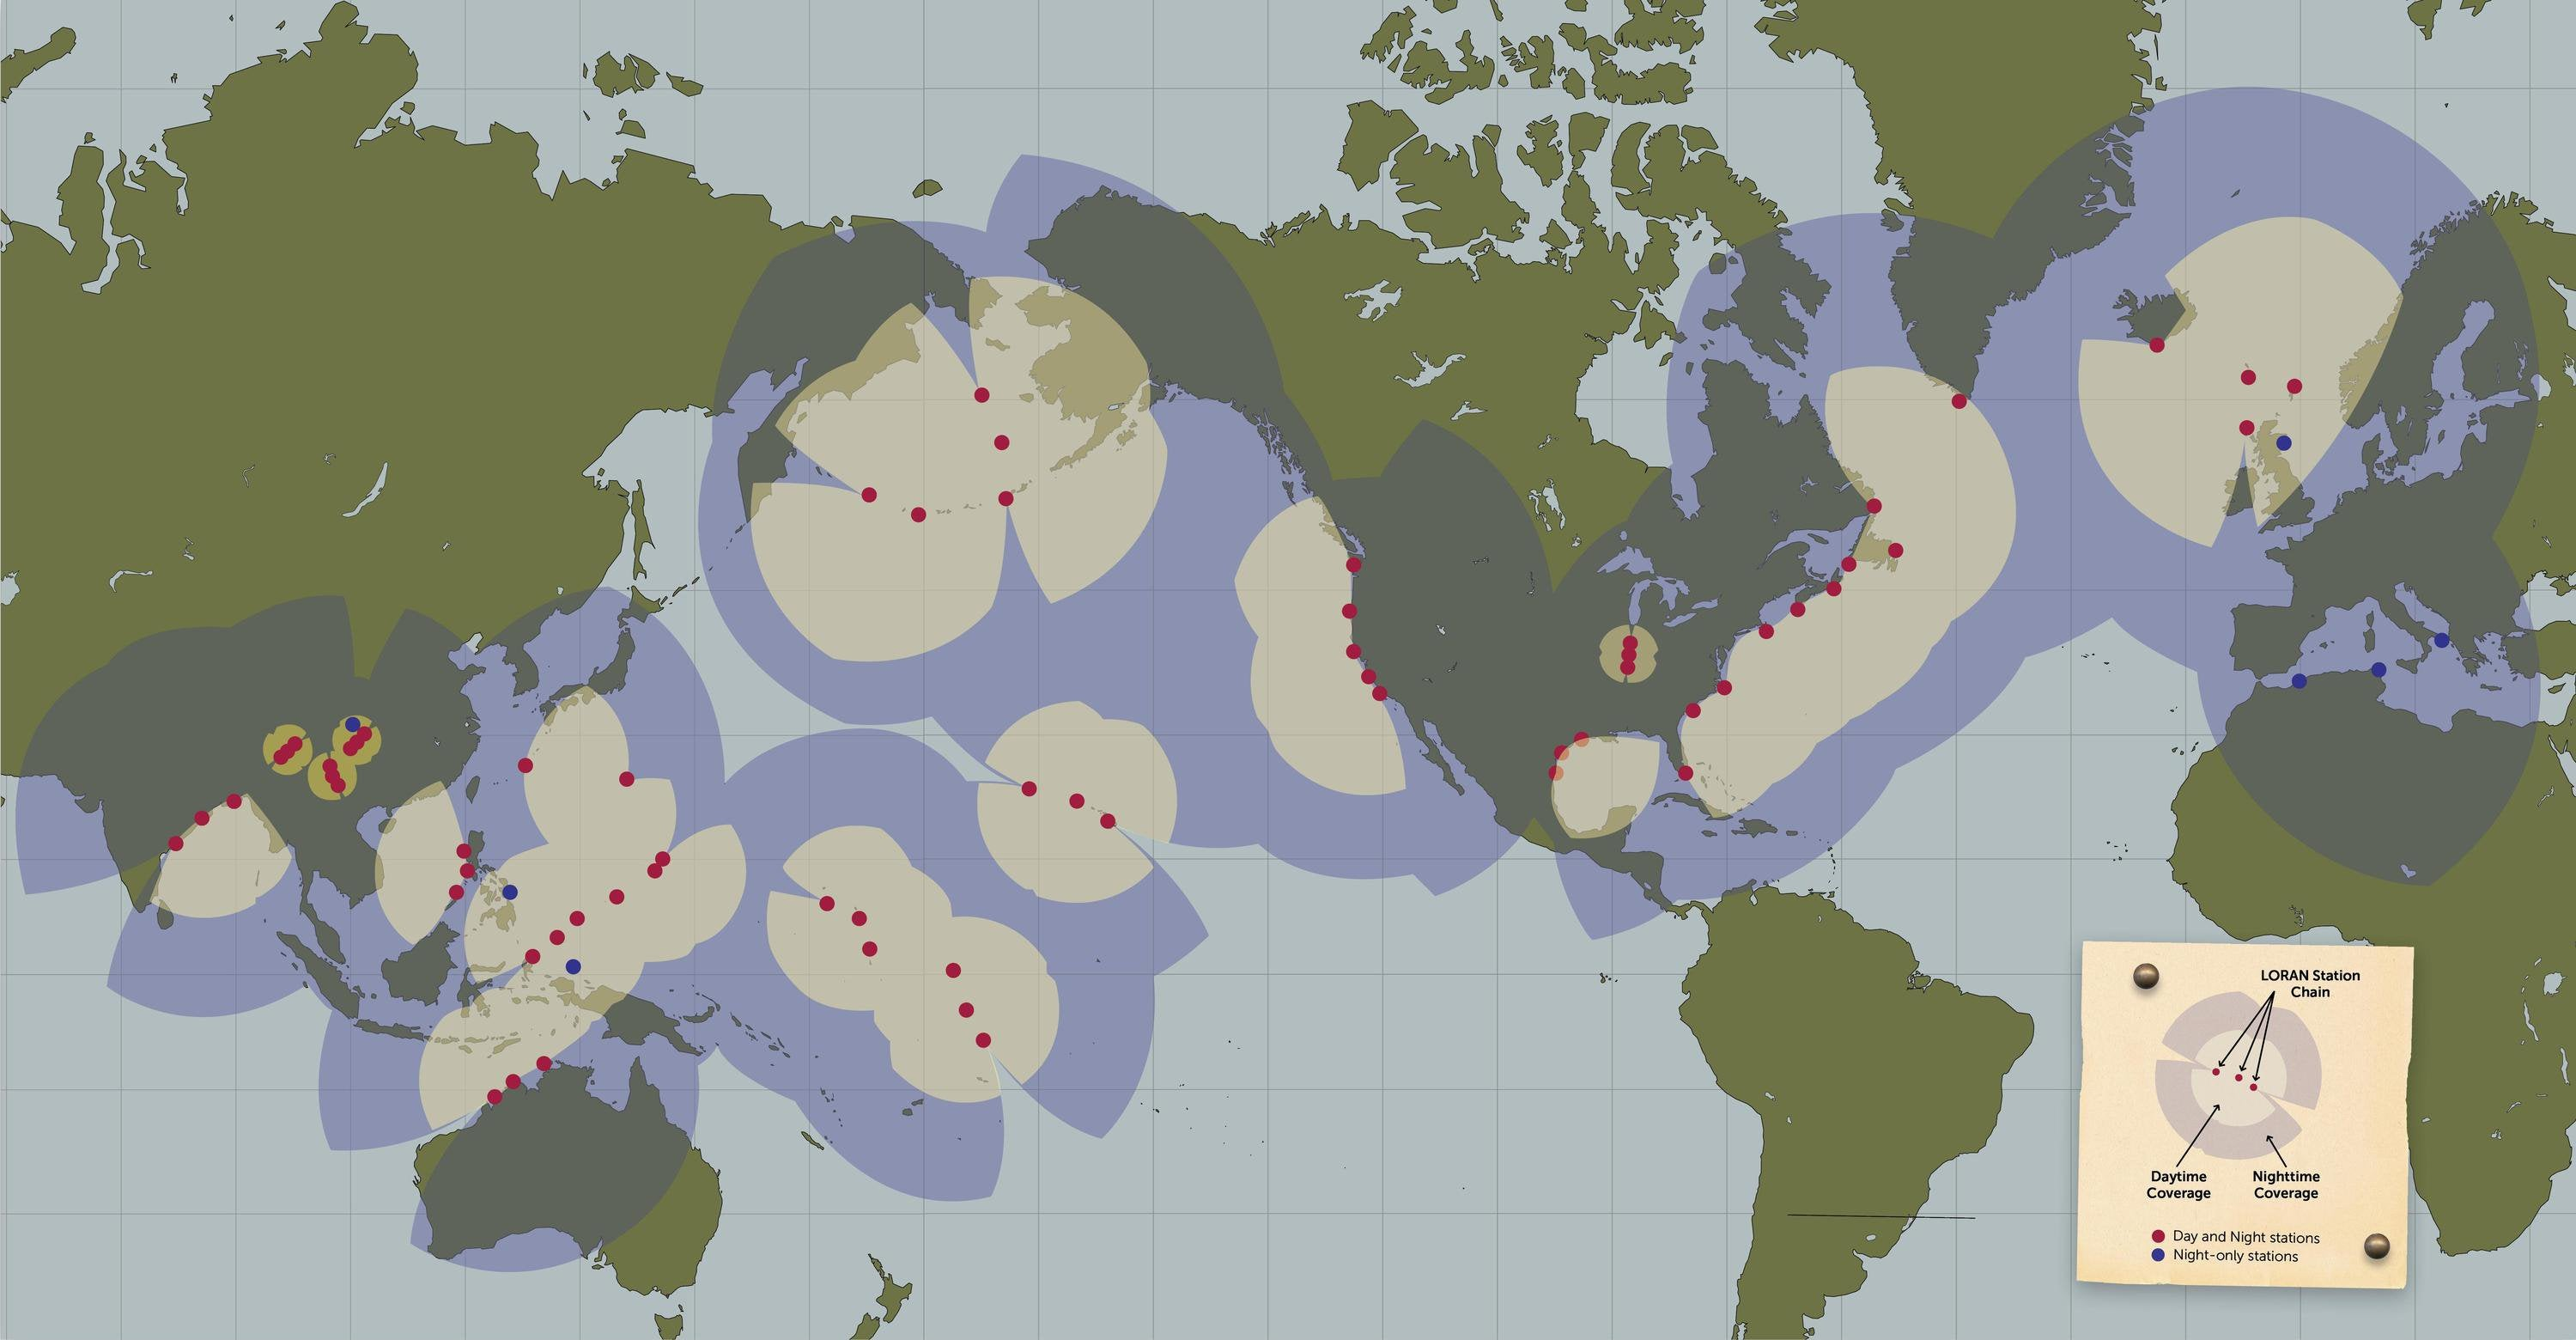
\includegraphics[width=\textwidth]{06.radionavegacion/Imagenes/06.01.Loran/06_Loran_cobertura.jpg}
    \caption{ Cobertura LORAN.  
{\scriptsize Fuente: \url{https://www.reddit.com/r/MapPorn/comments/3aaak8/station_location_and_coverage_areas_of_the_loran/}}     }
    \label{fig:LORAN-A-cobertura-1973}
  \end{figure}

\end{landscape}



